\chapter{Litterature Review and Analysis}
% !!!
%In this section, we will review the state of the art and the related work that has influenced our approach. First, we review the contact profile in different applications in section \ref{contactprofile}. Second, we investigate contact relationships in popular social networks in section \ref{contactrelationships}. In section \ref{cloudcontact}, we discuss the cloud-based Contacts application and its potential. Lastly, we examine 3 database schemas which are designed for a tagging system in section \ref{databasedesign}

\section{Contact Information and The Need of Tagging}\label{contactprofile}
Most of our daily communication activities involve managing contacts information. Through a field study from Whittaker et al. \cite{Whittaker2002} the value of contact information is strongly affirmed. Mary, a participant in the field study stated that her personal contacts list was a resource which pervaded all of her work:

``I cannot work today unless I have some source of contact information, some organized source so I can actually actively search for people. I use this list all the time just to browse it to find people when I need somebody to do a particular task.''\cite{Whittaker2002}

Understanding the importance of the contacts list, Jung and other researchers at Nokia \cite{Jung2008} introduce eight design drivers a Contacts application should follow:

\begin{enumerate}
  \item \textbf{Efficiency of accessing contacts}: Apparently, speed and ease of accessing and creating new contact information are key factors of the Contacts application. They should be the first priority in the design process.
  \item \textbf{Differentiating important contacts}: Interviewed participants in Jung et. al. study expressed their demands in differentiating special contacts from others for both emotional and practical goals. As the size of mobile contacts list grows, many participants manually changed the order of appearance of some contacts in the list (for example, by adding a number ``1'' in the name field) or attaching a visual mark to make the contacts stand out of the list (for example, adding symbols like ``*'' or a heart ``<3'' to indicate his/her significant other). However, the nature of relationship often changes over time so manually altering contacts as shown above is obviously tedious and not ideal. Therefore, on a practical level, the researchers recommend using a dynamic list which can be automatically generated based on some conditions like frequency and recency of communication to differentiate important contacts.
  \item \textbf{Customization and personalization}: Jung et. al. claim that the Contacts application is a highly personal application which accommodates different user preferences and lifestyles. Hence, it is essential to have a model to understand the range and patterns of user preferences which can be interpreted into user preference settings. The researchers then propose the feature that allows personalization of content on various levels such as adding a picture, an icon, a note to a contact profile.
  \item \textbf{Contact as repository of personal information}: Nokia researchers show that contacts list is not only about other people. Their interview revealed that users store personal information which is unrelated to communication management in their Contacts application. This information could be passwords or account numbers or other data that may potentially be retrieved more than once. Some advanced users developed some special ways to ``encrypt'' their private data to make it secure (for example, naming the credit card PIN number as ``Jonny'' in the contacts list). In addition to users' own personal information, through their study, the researchers found it is necessary to promote users storing others' digital identities in the Contacts application. 
  \item \textbf{Contact as social piggy bank}: People often consider adding other information which is related to the social relationship to the contact profile if the application has that functionality. Active users in Jung's study wished to have the ability to add further information about the person such as birthday, social network, communication history to provide or strengthen the context of the relationship, especially when the user has a strong social connection with the person. Therefore, it is essential to design a contact profile that can accommodate both the people-centric and the information-centric types.  
  \item \textbf{Assistance to social management}: The study revealed different areas where people will benefit from making use of past communication patterns (for example, storing the date of when the contact profile was created, which may mark the moment when the user first met that person). In contrast with the ``Contact as social piggy bank'', this design driver helps users who do not proactively add extra information since most data of this kind could be accumulated and stored automatically.
  \item \textbf{Flexibility in organization}: Jung et. al. stated that their research revealed various potential reasons why people may use hierarchical or grouping organization in the contact profile. One of the reasons was to assign common settings like special ringing tone to a group of contacts. Another reason was to assist faster access and reduce the visual clutter when there were many contacts with the same names.
  \item \textbf{Accessing external contact information}: With the powerful mobility of mobile phones, sometimes accessing the basic information of a foreign area is necessary in an unexpected circumstance (for example, taxi, hospital, directory service). Therefore, it is desirable to have access to the locally related data. The researches suggested that instant access to external contact information database has a big potential in improving the Contacts application.
\end{enumerate}

The design drivers listed above were published in 2008, one year after the first iPhone flipped the world upside down by introducing a whole new concept of touch-screen smart devices. Over the years, these drivers have been proven to be applicable and implemented completely or partially by manufacturers. Taking a look back into the past, the first Contacts application on a mobile phone was simply a dictionary of names and numbers. A contact profile used to consist of only the person' s name and his/her phone number. Nowadays, a contact profile in major platforms (iOS, Android, Windows Phone) is not only the person's name and phone number but also their social profile. This social profile is made up of the person's picture, name, phone numbers, and a group of miscellaneous fields such as company, job title, address, birthday, emails, notes, and so on. Furthermore, the Contacts application provides users with many extra functionalities such as logging communication history, marking favorite contacts, grouping contacts. We can see that almost all the design drivers are implemented in modern Contacts application except for design drivers number 4, 8, 3 and 6. As a side note, we do not sort the design drivers by numerical order here but we sort it by its content explained below:

\begin{itemize}
  \item \textbf{Design driver number 4 - Contact as repository of personal information}: At the time Jung et. al. proposed the design drivers, smart phones were not yet powerful. Therefore, it is understandable that some people utilized the Contacts application to store their personal information like account number, usernames, passwords. However, with the capabilities of modern mobile phones, users have many choices to accomplish that task. For example, it is much better to save private information using a password manager application since it is more convenient and the data is safely protected using modern encryption algorithms. For other kind of information, users can choose to store it in a note taking application or a task manager which are available on all mobile platforms. In summary, this design driver has become inappropriate in today technologies.
  \item \textbf{Design driver number 8 - Accessing external contact information}: Having the ability to retrieve external and location-related information directly from the Contacts application is desirable. However, the enormous power of today search engines together with the rising of mobile intelligent personal assistant like Siri (iOS), Google Now (Android), Cortana (Windows Phone) has made accessing external information incredibly easy. Users can just verbally command the intelligent personal assistant or type a few keywords in an on-screen widgets then the relevant information will be retrieved instantly from a search engine. Therefore, the majority of users has developed a habit of looking up for external information via search engine, hence using the Contacts application for this task becomes redundant and sometimes slow. To conclude, accessing external contact information from the Contacts application has turned out to be just a ``nice to have'' feature without much potential thus not being implemented in most modern Contacts applications. 
  \item \textbf{Design driver number 3 - Customization and personalization}: Unlike the two obsolete design drivers we have just analyzed, design drivers number 3 and 6 are actually implemented in almost all Contacts applications today. Design driver number 3 is about customizing and personalizing the contacts. In modern Contacts applications, this driver exists in the form of the picture in the contact profile and a group of extra fields like websites, phonetic name, notes. However, all those fields are pre-defined by the application. To the best of our knowledge, all Contacts applications lack the ability for adding customizable fields. In other words, we consider the pre-defined fields only fulfill the ``Personalization'' half of design driver number 3 while missing the first half - ``Customization''. In 2010, Trung V. Nguyen et. al. \cite{tagging} conducted a survey with the participation of 87 people in Korea which revealed that Contacts application users need various extra customizable information related to a contact. They then pointed out that memos or notes are not sufficient for this purpose, and proposed the use of tags. We are totally in unison with this idea of using tags for customization and we will discuss more in details of this topic in section \ref{section:Tagging}.
  \item \textbf{Design driver number 6 - Assistance to social management}: Assistance to social management is another limitedly implemented design driver. From our analysis, all major Contacts applications today only record the calls and text messages log of a contact while there are many more potential past communication patterns. For example, the date and the location a contact was created may tell a lot about how the user meets that person. The survey from Trung V. Nguyen et. al. \cite{tagging} shows that many people struggle with remembering who the contacts are and who they should call for a piece of information. In these situations the past communication patterns can be very helpful. We will analyse this problem more in section \ref{section:Context_Awareness}
\end{itemize}

\subsection{Tagging}
\label{section:Tagging}

Tagging is using keywords to add metadata to content \cite{golder2006usage}. It has become very popular in applications and services nowadays \cite{cattuto2007semiotic, golder2006usage, marlow2006ht06}. Many types of data are currently annotated by tags which includes bookmarks, images, videos, articles, blogs and so on. There are different services providing tagging functions to data such as Pocket, Pinboard, Delicious, Flickr, Youtube. Tagging is effectively enhancing users experience in organizing and sharing large amounts of information in those services.

In order to understand tagging, Ames and other researchers at Yahoo and Stanford University conducted a large study on more than 500 people \cite{ames2007we}. The study focused on an images tagging system combined of Flickr and ZoneTag. Flickr is an image hosting web services. It is a popular website having one of the largest online communities. Flickr provides annotation of images in the form of tags. A tag in Flickr is an unstructured textual label and mainly assigned by the user who owns that image. ZoneTag is a mobile application developed by the researchers. It helps users upload a newly captured photo from their mobile phones directly to Flickr in just a few clicks. More importantly, the users can type in or select tags for that photo. This feature pre-fetches a number of tags from the ZoneTag server based on the context then suggests them to users for easy selection. ZoneTag was deployed as a public prototype for around a year with more than 500 users and 45,000 uploaded photos. Ames et. al. then carried out a study on 172 users. During the deployment process, Ames collected their data about the usage of the system. The data was used to analyze tagging patterns and activity. Figure \ref{fig:zonetag} demonstrates the percentage of users regarding their average number of tags per photo. For instance, the first bar on the left indicates that 25\% of the ZoneTag users have less than 0.5 tag per photo. Notably, this number does not count the automatically added tags. As we can see from the chart, around 61\% of the users added at least one tag for each photo on average. Surprisingly, over one fifth of the users had more than 3 tags per photo which reveals a great potential of tags. All the tags of the system come from ZoneTag mobile application as well as Flickr's official website. However, the majority of tags were from ZoneTag with over two thirds of the tagged photos were added by users with their mobile devices.

\begin{figure}[!h]
\begin{centering}
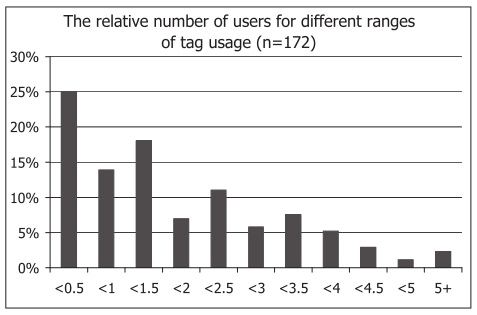
\includegraphics[scale=0.7]{pics/zonetag.png}
\caption{ZoneTag users' tagging frequency across their entire Flickr collections (including untagged photos)}\label{fig:zonetag}
\end{centering}
\end{figure}

In addition to analyzing collected data from users, Ames et. al. conducted an in-depth, semi-structured interview with 13 participants including some users who had taken the most photos. Their ages ranged from 25 to 45 with four of them being female. The tagging frequency of each participant covered from zero to more than five tags per image. The interview revealed many type of motivations and uses of tags. Almost all the participants had more than one motivations for tagging. For example, an interviewee tagged her photos in order to retrieve them later as well as to provide contextual information of the images for herself and her friends. The researchers established a taxonomy for the motivations which included 2 categories and 4 groups:

\begin{itemize}
    \item \textit{Self/Organization: Search and Retrieval}
        
        This is the traditional motivation of tagging. Users who have this motivation occasionally make comments like ``I am an organized person'' or ``I like order''. However, these comments are often followed by admission for not being consistent in the tags. Two of the participants say that they tag especially to later retrieve their photos and two others say they tag for personal organization purpose. Below is the quote from one of these participants:

      ``Mostly I use tags if I go back on Flickr if I want to find all the pictures of one thing. If I tagged ahead of time I can go back and get all my pictures of my children.\ \ldots \ I've made separated tags of my child's preschool or playgroup so that if I want to share pictures with more than just family I can go back and find everything from that one tag. \ldots \ Mostly it's for my own organization at this point.''

      \textbf{Analysis}: This traditional motivation is totally appropriate with a Contacts application. In order to improve users' consistency we should provide a good tag suggestion/recommendation mechanism.

  \item \textit{Self/Communication: Memory and Context}
      
      Users sometimes add tags to give context to a photo like the names of the people in it or the location that photo was taken. This behavior improves future recall of the situation the photo illustrates. However, it is surprising that not many users were motivated in this way when they tagged their photos. The quote below demonstrates a user's perspective:
      
      ``If I have the time, the neighborhood, or the event, I have enough information to look at my own collection and know where this came from. I don't have the bandwidth to tag for the benefit of the Flickr system\. \ldots \ I want at least one hook of association in there that can help me reconstruct what I was thinking. I don't have time to put all the hooks in but I can put one in.''

      \textbf{Analysis}: According to the study, there are only a few people having this motivation. From our point of view, there are two problems here. First, context information is ambient data so having it together with the primary data (photos, contacts) is always good so long as it does not distract the viewing process. However, adding ambient data is time consuming and often not appealing, hence not many people spend time doing it. Therefore, this kind of data should be added automatically by the application itself and provide them when needed. Second, a photo provides a lot of ambient information like the people in it, where it was taken. Just by looking at a photo, viewers can understand much about the situation surround that photo. On the other hand, a contact in the Contacts application does not tell a lot about itself. Thus, having ambient information in a contact can help user to recall things about that contact like where and how they met. It is really useful in case there are more than two contacts having the same name. In conclusion, we think this motivation is appropriate with a Contacts application and needs to be implemented properly. Another thing we wish to emphasize is sometimes it is not clear to differentiate a tag is the first type (Search and Retrieval) or the second one (Memory and Context). Therefore, to be consistent, we consider the second type (Memory and Context) always ambient data which is automatically added by the application.
      
  \item \textit{Social/Organization: Public Search and Photo Pools}

      This group represents the users' motivation for making their photographs searchable by other people. The researchers point out that pictures are often taken to enhance and document mutual experience or to share it with friends, family, and even the public. The tags can make the photos be easily found by people the users want to share with or anybody who is interested in them. While some users tag for their friends and family, other users tag for the general public. Below is the quote about this aspect:

      ``Most friends view my photos, but as I grow my collection, I am getting more public views. I've noticed that if I take and tag pictures of cute female friends, views go up.\ \ldots \ There's a satisfaction that 50 people have viewed my photos. I know that tagging can connect my photos to activities, and get more interest. \ \ldots \ I got more liberal about using suggested tags lately, so I will add multiple tags to make it easier for people to find my photos.''

      As more users tag their images, appealing behaviors arise between groups of friends. Two of the participants said that they coordinated tags with others to assist later retrieval. This is a form of an ad-hoc, distributed photo ``pool''. One participant did this with his friends in many situations like company meetings, parties, classrooms or hikes with friends. Another participant attended a race in San Francisco then he utilized the tags that others were using to tag his own pictures as well as finding other photos of the event. The quotes reflecting these behaviors are listed as follows:

      ``I'm at an event and there's a convergence on a specific tag, then I'll tag because it's for the good of the group. \ \ldots \ It's a nice way to build live streams and collections of photos. \ \ldots \ A classmate suggested we tagged everything specifically so we can find it, which is actually really useful.''

      ``If I'm out with friends they might suggest tags.\ \ldots''

      \textbf{Analysis}: This motivation is not exactly relevant to a Contacts application since the contact information is generally private and often not shared with the general public. However, ad-hoc sharing is an interesting aspect our Contacts application can learn from Flickr and ZoneTag. Sharing a contact with its tags and additional contextual information might be helpful to the receiver since he/she will probably have sufficient contextual knowledge to understand the tags. Nevertheless, this feature should be designed with care because tags often contain a great amount of personal information which the author may wants to keep for only himself. That is why, the ability to select which tags to be shared is essential in this feature.

  \item \textit{Social/Communication: Context and Signaling}

      The last group is tagging to communicate contextual data to other users. In almost all cases, users added these contextual tags for friends and family. Contextual tags for known people often have little meaning for the public. Actually, in order to improve privacy, some users confuse their tags on purpose to make it impossible for the general public to understand the tags. Additionally, two participants described tagging as ``a chain reaction'', when somebody took a photo and tag, others also took out their phone. One participant describe this perspective as follows:

      ``I tag and I don't have to explain myself - my friends don't have to ask me a billion questions such as `where did you take this photo, why are you showing me this photo, who is this person in this photo'\ldots \ I can give them the basic story.''

      \textbf{Analysis}: This is another motivation with little relevance to our Contacts application. Since the contact data is not exposed to the public, we do not have to worry much about privacy issues. However, the ``chain reaction'' is a good sign from which we can believe that tagging in a Contacts application can be widespread.

\end{itemize}

From the interview, Ames et. al. also analyzed the best way to design the tags suggestion feature. First of all, the researchers decided to make interactions between users and the main activity as burden-free as possible. Particularly, ZoneTag was designed to do its main job in only 2 clicks and it did not require users to add or select tags right away. The reason behind not making adding tags mandatory is that many users from the interview found it difficult to add or even select tags on the phone in some situations like driving or socializing, furthermore, even participants who added many tags still did not want to be interrupted all the time. Secondly, many participants liked having previously-used tags showed up and they also used the auto-completion feature widely. However, the researchers also found out that tags sometimes confuse the users when they share them with each other. One participant complaint about an unfamiliar tag on her photo after using the tags sharing feature in a conference. Nevertheless, from our point of view, sharing photos and sharing contacts are very different since we often share a much smaller set of contacts with just one or two people so the confusion should not be a problematic issue. Lastly, Ames et. al. discovered that tags suggestions served a larger purpose than just assisting in tag entry. Some users had developed the habit of browsing the suggested tags list to add all the tags which were relevant even if they did not try to add them in the first place. One participant commented that he often scrolls down the list and picks available tags because they are displayed. Moreover, even when not being selected, the suggested tags still encourage some participants to add their own new tags and give them direction to the types of tags they may use (for example, a suggested tag about a neighborhood may inspire the users to add tags about other neighborhoods as well). In summary, tags suggestions have a significant impact on users' tagging activity, however the option to bypass adding tags in some circumstances is important for the usability of the whole system.

In the end of the study, after carefully analyzing users' data as well as the interview, Ames et. al. summarized their findings into a list of implications for the design of tagging systems in general \cite{ames2007we}:

\begin{itemize}
    \item Make the annotation ubiquitous and multi-functional.
    \item Make it as easy as possible when the data (photos, contacts\dots) is captured.
    \item Do not force annotation at the point of information capture.
    \item For systems that have both mobile and desktop or web-based components, annotation should be enabled in both settings.
    \item Relevant suggested tags can inspire tagging and direct users to possible tags.
\end{itemize}

We have just examined principles of a general tagging system, we will now investigate how tags should be applied on the mobile phone's Contacts application. In 2010, Nguyen et. al. conducted a user study \cite{tagging} to discover users' dissatisfactions with contacts management. The study consisted of a large survey which incorporated multiple choice and open-ended questions so participants could point out changes they wanted to be made in their current Contacts application. The survey focused on finding the issues with storing, searching and managing the contacts. It was conducted through an online form over the course of one week with the participation of 87 people. There were 42 male and 45 female participants and their ages ranged from 15 to 50. First, the survey asked participants on the way they organize their contacts. 46 participants said that they use groups for organization while 42 participants did not. However, almost everyone thought that classify the contacts using groups was inconvenient. 55 participants did not know which group they should put a contact into, 12 had difficulty finding appropriate names for their groups, and 11 people claimed that they could not search for contacts using group names. The issues were revealed more clearly through the open-ended questions from which 5 people wanted to put a contact into various different groups while 4 other participants wanted to have hierarchical groups. From these answers, Nguyen et. al. concluded that people use groups as a way to label multiple pieces of information of a contact which may help them recall and fetch the contact when needed. Furthermore, the researchers also addressed the problem when people forget about contacts they have created earlier. 45 out of 87 users said that they did not know who they should call for a piece of information. The problem became more serious when it passed on to business service contact information. Business service such as restaurants, childcare, repair and maintenance, transportation are actually really important. They are the kind of long-term interaction which are infrequent but long-lasting contacts. The survey revealed that 47.5 percent of the participants call this kind of service contacts at least once a month and more than three quarters of all participants call more than once every three months. Despite the importance of these contacts, participants often struggled to look for service numbers in their mobile Contacts application. Among 87 people, 61 did not remember whether they had stored the demanding contact or not, 40 did not recall the name they used when created the contact, and 21 had to look through the entire contacts list to find the number. This fact undoubtedly indicated the need of a system which can assist users in finding the right contact when they have some particular pieces of information about the person/service.

The study also disclosed several solutions which users created manually by themselves in an attempt to tackle those problems. 7 users used memos or notes to store extra information about their contacts while some others put the information into the name entry of contacts just like the way participants in Whittaker's study did which we have examined in the beginning of section \ref{contactprofile}. From this revelation, Nguyen et. al. concluded that users need an efficient mechanism for storing and retrieving extra information of a contact. Therefore, the researchers proposed the use of tags which were convenient for adding and searching resources. Resources could be classified by numerous tags rather than using a directory or a single branch of hierarchy \cite{millen2005social}. As a result, users could ``tag'' a contact into multiple groups or even made the tags hierarchical based on their needs. Regarding retrieval, multiple tags could be used simultaneously in a query for a specific contact so the users did not have to remember the person/service name.

\begin{figure}[!h]
\begin{centering}
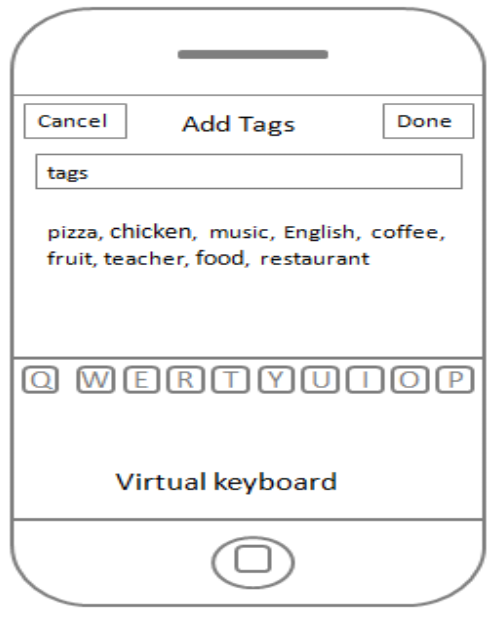
\includegraphics[scale=0.5]{pics/paper_prototype_1}
\caption{Nguyen et. al.'s ``Add Tags'' UI on A Paper Prototype \cite{tagging}}\label{fig:paper_prototype_1}
\end{centering}
\end{figure}

\begin{figure}[!h]
\begin{centering}
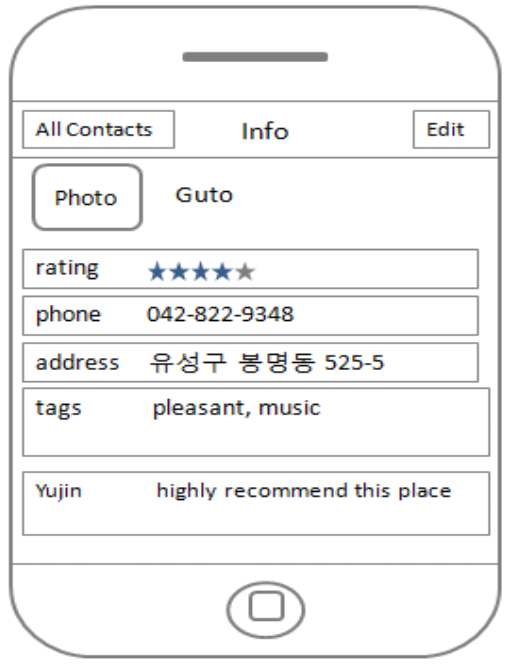
\includegraphics[scale=0.5]{pics/paper_prototype_2}
\caption{Nguyen et. al.'s ``Contact Info'' UI on A Paper Prototype\cite{tagging}}\label{fig:paper_prototype_2}
\end{centering}
\end{figure}

After conducting the survey, Nguyen et. al. created a paper prototype of a mobile phone Contacts application to verify their findings. The paper prototype was used in various user study scenarios. At the start of each scenario, the researchers explained to the users new features in the Contacts application. After that participants were requested to perform tasks by interacting with the paper prototype. A researcher acted as the application by responding to users' interactions with other user interfaces also on papers. Figures \ref{fig:paper_prototype_1} and \ref{fig:paper_prototype_2} are two example user interfaces of the paper prototype. After finishing a task, the participant filled in the task assessment form and answered some questions from the researchers. All participants thought the tasks were realistic and they had come across many times in real lives. They also commented that the tasks covered all the information they needed when using the Contacts application. In general, the participants had positive feedbacks about the prototype. For instance, a user liked the tagging feature and actively used it a lot through out the scenarios. Furthermore, most of the users only used the name of the service as search keyword once every 20 scenarios, instead they often looked up the contact by using information from the scenarios which were remarkable, relevant, and personal. This was a definitely good sign which indicated the capabilities of tags in directing users to the right contacts from miscellaneous information. On the other hand, some participants admitted that they are sometimes too lazy to enter text on their mobile phones even though they knew that some information about a contact was absolutely necessary. This issue again pointed out the importance of tags suggestion which we have already covered in previous sections.

\textit{\textbf{Summary}}: To sum up, we have comprehensively investigated a study about tagging in general and another study about tagging in a mobile Contacts application. Both studies suggest that tagging is an essential aspect which could help users organize their data. From Flickr/ZoneTag, we understand the motivations behind tagging, and the recommendations from the researchers will direct us when we build our own system. From the study in Korea, tagging in a Contacts application is once more affirmed to be necessary, and the paper prototype is really helpful for us in designing our application's user interfaces.

\subsection{Historical Contexts Awareness}
\label{section:Context_Awareness}

As we have discussed at the beginning of this chapter, the design driver number 6 - Assistance to social management is not fully implemented in Contacts applications nowadays. In order to utilize this design driver, we propose the use of past activities in the form of historical contexts. The contexts here can be many aspects around a contact which happened in the past (this is the reason why we use the term ``historical contexts'' to distinguish them from the ``current context'' which is often used to determine the status of the users). For example, the location and the date/time when a contact is created are useful historical contexts which can tell a lot about the situation when the user met that contact, and the events, meetings happened around that time, other contacts added just before and after that contact are meaningful pieces of information as well. Furthermore, the communication history between the user and a contact via emails, call log, and social network interactions can also be considered valuable historical contexts. With the assistance of historical contexts, users can use their Contacts application to recall memory about a contact when needed. Looking back at our analysis of Ames' tagging motivations in section \ref{section:Tagging}, memory and context is the second motivation of tags. Therefore, we decide to make historical contexts a kind of tag in our system. This kind of tag will be automatically included into a contact profile of the Contacts application along with users-created tags. To understand more about historical context, in this section we will first investigate the definition of context, design principles for context-aware systems, then we will examine ``Forget-me-not'' an intimate computing system which use context to support human memory.

According to the survey from Baldauf \cite{baldauf2007survey}, the term ``context-aware'' first appeared in Schilit and Theimer's work in 1994 \cite{schilit1994disseminating} in which the authors defined context as locations and identities of nearby people and objects. In 1998, Ryan \cite{ryan1998enhanced} referred to context as the user's identity, surrounding environment, location, and time. From another angle, Dey \cite{dey1998context} not only described context as location, time, and user's environment but also as user's emotional state, focus of attention. However, in the opinion of Baldauf, the most accurate definition of context was given by Dey and Abowd \cite{abowd1999towards} as ``any information that can be used to characterize the situation of entities (i.e., whether a person, place or object) that are considered relevant to the interaction between a user and an application, including the user and the application themselves.'' Regarding context classification, a common way to organize context is based on its dimensions. Prekop et. al. \cite{prekop2003activities} and Gustavsen \cite{gustavsen2002condor} classified the dimensions into external and internal. The external dimension is the physical context which can be calculated by hardware like location, time, and movement. The internal dimension is the logical context which can be measured only by the users themselves or captured by monitoring users' interactions. Some examples of internal context are the users' tasks, work context, or the users' emotional states. All most all context-aware systems utilize external context since they give valuable information while being easy to measure using modern hardware sensors. There are also some systems making use of logical context like Watson \cite{budzik2000user} and IntelliZap \cite{finkelstein2001placing} that assist users by presenting relevant information based on information extracted from users' opened web pages, and documents.

When designing a context-aware system, the method to capture context information is crucial since it greatly influences the architecture of the system. Chen et. al. \cite{chen2003ontology} demonstrated three different ways to capture context information.

\begin{itemize}
    \item \textit{Direct sensor access}: This method is widely implemented in hardware devices with built-in sensors. The software collects the needed contextual data directly from the sensors, hence, no extra layer for gaining and processing sensor data is required. However, drivers for those sensors are attached to the application layer forming a tightly coupled system which is not flexible. As a result, this approach is not suitable for distributed systems because of its direct access nature.
    \item \textit{Middleware infrastructure}: This method divides context-aware systems into layers. The main purpose of this approach is to hide low level sensing details. In comparison with the first method, this layered architecture approach is more flexible and extensible. The application layer is separated from the sensors so it is easy to reuse hardware dependent sensing code. However, the architecture is more complicated compared with direct sensor access.

    \item \textit{Context server}: This method expands the middleware approach by introducing a remote server. This server aggregates sensor data then provides access to authorized clients. The first advantage of this technique is reusing sensor and introduce an administration layer for the contextual data. The second advantage is saving the clients from resource intensive operations since almost all client devices in a context-aware systems are mobile devices with limited computing power, memory, and energy. On the other hand, this approach requires a complex communication protocol between clients and the server, and the network performance can sometimes become the bottleneck of the system.
\end{itemize}

Regardless of what method a system chooses to capture contextual data, logically separating context detection and context consumption is essential in enhancing extensibility and reusability of the system. Figure \ref{fig:context_aware_systems} illustrates the layered logical architecture which was described by Ailisto et. al. in 2002 \cite{ailisto2002structuring}.

\begin{figure}[!h]
\begin{centering}
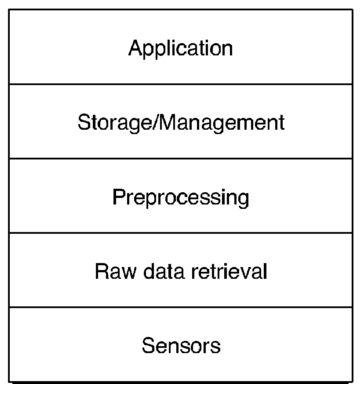
\includegraphics[scale=0.6]{pics/context_aware_systems}
\caption{Layered Conceptual Framework for Context-aware Systems \cite{baldauf2007survey}}\label{fig:context_aware_systems}
\end{centering}
\end{figure}

The first layer is called the ``Sensors'' layer. The term sensors here not only means physical hardware sensors but also means any kind of data source that supplies valuable contextual information. In accordance with Indulska and Sutton \cite{indulska2003location}, sensors can be categorized into three different groups based on the way they capture data.

\begin{itemize}
    \item \textit{Physical Sensors}: This is the most common type of sensors. They are the actual hardware sensors that can capture many kinds of physical information like longitude, lattitude, temperature\ldots. Physical sensors are very popular today and can be found in almost all smart devices or mobile phones. Table \ref{tb:sensor_types} lists some common physical sensors.
    \item \textit{Virtual Sensors}: This type of sensors get contextual information from software or services. For instance, an application can track users' location not only by using GPS data but also by reading their electronic calendar, emails. 
    \item \textit{Logical Sensors}: Logical sensors take advantage of multiple data sources by incorporating physical and virtual sensors with supplementary information from databases or other sources to deduce more complex information. For instance, logical sensors can be used to track employees' current location by examining user logins on company's machines and combine those pieces of information with a database storing machines' locations.
\end{itemize}

\begin{table}
    \centering
    \begin{tabular}{ | l | p{7cm} |}
    \hline
    \textit{Type of Context} & \textit{Sensors} \\ \hline
    Light & Photodiodes, color sensors, IR and UV sensors, etc. \\ \hline
    Visual & Cameras \\ \hline
    Audio & Microphones \\ \hline
    Motion, acceleration & Mercury switches, angular sensors, accelerometers, motion detectors, magnetic fields \\ \hline
    Location & Outdoor: Global Positioning System (GPS), Global System for Mobile Communications (GSM); Indoor: Active Badge system, etc. \\ \hline
    Touch & Touch sensors in mobile devices \\ \hline
    Temperature & Thermometers \\ \hline
    Physical attributes & Biosensors for measuring skin resistance, blood pressure, etc. \\ \hline
    \end{tabular}
    \caption{Commonly Used Physical Sensor Types \cite{baldauf2007survey}} \label{tb:sensor_types}
\end{table}

The second layer, \textit{Raw data retrieval}, is for retrieving raw contextual data. It utilizes drivers on physical sensors or APIs on virtual and logical sensors. This layer provides abstract functions for the upper layer in order to make it easy for accessing the low-level hardware layer. Furthermore, by abstracting the access interfaces, it is possible to replace the hardware sensors module with another one without changing the upper layer's program. For example, replacing a RFID sensor with a GPS one can be done seamlessly.

The third layer is not commonly implemented in context-aware systems. It is used for interpreting context information which is sometimes important when the raw data is too harsh. In some systems, the technical data from the sensors is not directly useful for the high-level software application. This is when the preprocessing layer is brought into play, it transforms the data into higher abstraction information by using extraction and quantization operations. Moreover, in systems which have more than one context information source, the data of all sources can be aggregated in this layer before delivering to the next layer. The aggregation process is often important since in many scenarios the data from a single sensor does not make sense or is inaccurate while the combined data from multiple sources is valuable and much more precise.

The forth layer is called \textit{Storage and management}. It organizes and store the collected data then provides them through interfaces. The applications/clients can receive the data synchronously or asynchronously.

They highest layer in the stack is the \textit{Application} layer. All the business logic that makes use of the stored contextual information is carried out here.

The next important thing we need to know when designing a context-aware system is the context models. The context models represents the machine readable form of the contextual data. It is challenging to develop a scalable, adaptable, and usable model which can cover a broad range of potential contexts. In their work ``A Context Modeling Survey'' \cite{strang2004context}, Strang and Linnhoff-Popien listed the most common context modeling methods. These methods were categorized based on the data structure representing context data.

\begin{itemize}
    \item \textit{Key-value model}: This is the most simple data structure which can be used for modeling contextual information. Although this model is simple, it is very effective and is used in many systems. According to Strang and Linnhoff-Popien, it is especially used a lot in service frameworks in which the key-value pairs represent the capabilities of a service. As a result, service discovery can be applied by running matching algorithms on the key-value pairs.
    \item \textit{Markup scheme model}: This kind of model makes use of markup tags with attributes and content to construct a hierarchical data structure.
    \item \textit{Graphical model}: Graphical model mostly utilizes the Unified Modeling Language (UML) which can be used to model context data. Some graphical model also extends the Object-Role Modeling (ORM) to represent context.
    \item \textit{Object oriented model}: This approach can leverage the power of object oriented techniques like inheritance, encapsulation, etc. Various context types can be represented by different objects.
    \item \textit{Logic based model}: This model has a high degree of formality. Context models are defined by facts, expressions, and rules. After that, a logic system will manage those facts, expressions, and rules as well as allowing addition, update or removal of each element. Reasoning processes are used to develop new facts based on existing rules in the system.
    \item \textit{Ontology based model}: Ontologies are considered a potential way to model context data since they have a high level of expressiveness while maintaining the possibilities to apply ontology reasoning methods.
\end{itemize}

After investigating architecture and design principles of context-aware systems, we will now thoroughly examine Forget-me-not, a context-aware program used for Intimate Computing. Forget-me-not \cite{lamming1994forget} is a project attempting to find a method to assist human memory using mobile and ubiquitous computing. It aims to solve the problem of growing information load in daily life.

\begin{figure}[!h]
\begin{centering}
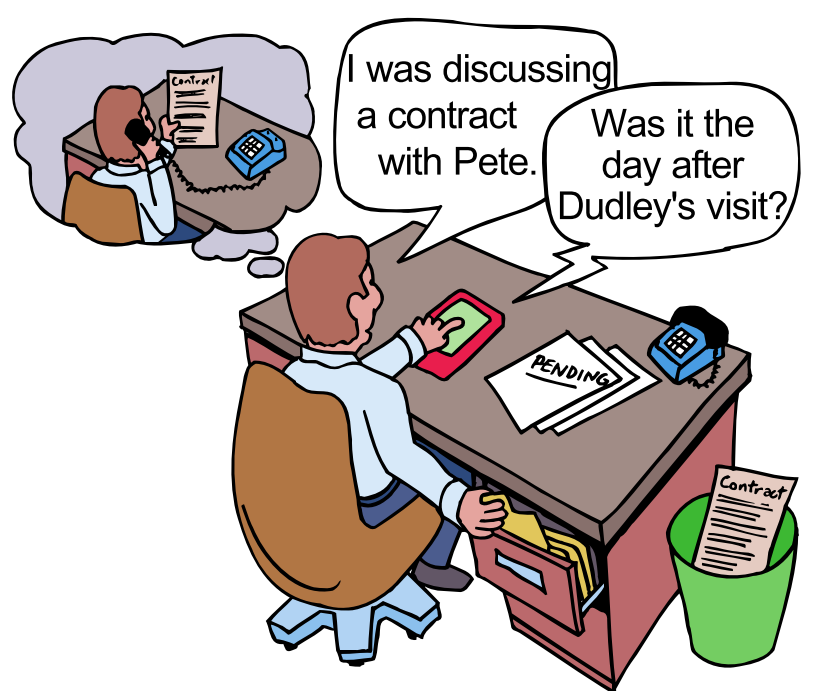
\includegraphics[scale=0.45]{pics/episodic_device}
\caption{Using A Prosthetic Episodic Memory Device \cite{lamming1994forget}}\label{fig:episodic_device}
\end{centering}
\end{figure}

In order to develop Forget-me-not, the researchers introduced a new computing model called ``Intimate Computing''. It was based on the definition of Ubiquitous Computing by Weiser \cite{weiser1991computer}, it consisted of tiny Personal Digital Assistants (PDAs) with wireless communication capability such as cell phones, laptops, wearable devices. Those devices always escorted the users so they can be tailored to their own preferences. Moreover, since they were involved in many of users' daily activities, the devices became intimate with them. The more intimacy the devices had, the more valuable they were. Furthermore, it is notable that Intimate Computing provided the computing devices with the users' real world contexts.

Utilizing Intimate Computing, the researchers attempted to solve the problem of forgetting one's own information. Since the PDAs had access to users' contexts, they could use the context as a useful key to index information automatically. According to the authors, a detail of a past event like the name of a document was probably hard for a user to remember. However, the context of that event could be easier to recall such as the person who gave the document to the user, the place when it happened, the task the user was doing. Psychology researchers also developed theories about this kind of physical contexts. They called it episodic or autobiographical memory. The psychologists discovered that people instinctively arrange memories of past events into episodes, and then the location of the episode, the people around, the activities that had happened before, during, and after the episode were solid clues for recall. Furthermore, a study by Eldridge et. al. \cite{eldridge1994autobiographical} even led us to believe that we could make a prosthetic episodic memory device. The device was called a \textit{memory prosthesis} which followed users and captured critical information and context from their lives, then it could organize this information into a structure which mimicked the episodic memories of human beings. As a result, people could retrieve details of their fading memories by looking up the episodes which were accumulated in the storage of their prosthetic memory devices (Figure \ref{fig:episodic_device}). In other words, users could use small, easy to remember things about a context to bring back the details that they had forgotten.

Forget-me-not was Lamming et. al.'s first attempt \cite{lamming1994forget} in creating a functioning prototype of a prosthetic episodic memory device. The first aspect of the device which the researchers tackled was user interfaces. They tried to design the interfaces to be as easy to use and intuitive as possible since it should be easier to remember how to operate Forget-me-not than to remember past events. Figure \ref{fig:forget_me_not} shows the Forget-me-not device developed in 1994. The software was implemented on a ParcTab - a portable device built in the Computer Science Laboratory at Xerox PARC.

\begin{figure}[!h]
\begin{centering}
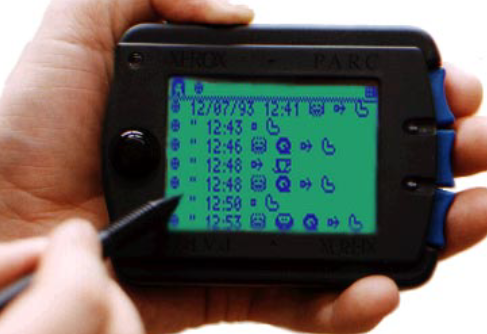
\includegraphics[scale=0.7]{pics/forget_me_not}
\caption{Forget-me-not Implemented on The ParcTab Hardware \cite{lamming1994forget}}\label{fig:forget_me_not}
\end{centering}
\end{figure}

By accompanying users, the ParcTab accumulated data about different users' activities then it arranged these data into a personal biography. In the simplest prototype, Forget-me-not required users to provide a list of devices where data could be gathered. When a user interacted with a device on the list, ParcTab automatically collected the device's name and location. The operations carried out by the user on that device were also collected together with a timestamp. When two people both wearing ParcTabs met each other, their devices would start exchanging information in regard to their preset privacy settings. Figure \ref{fig:intimate_computing} illustrates this model. According to the authors, the Forget-me-not prototype was deployed for a few months and to some extent confirmed the applicability of the Intimate Computing model. 

\begin{figure}[!h]
\begin{centering}
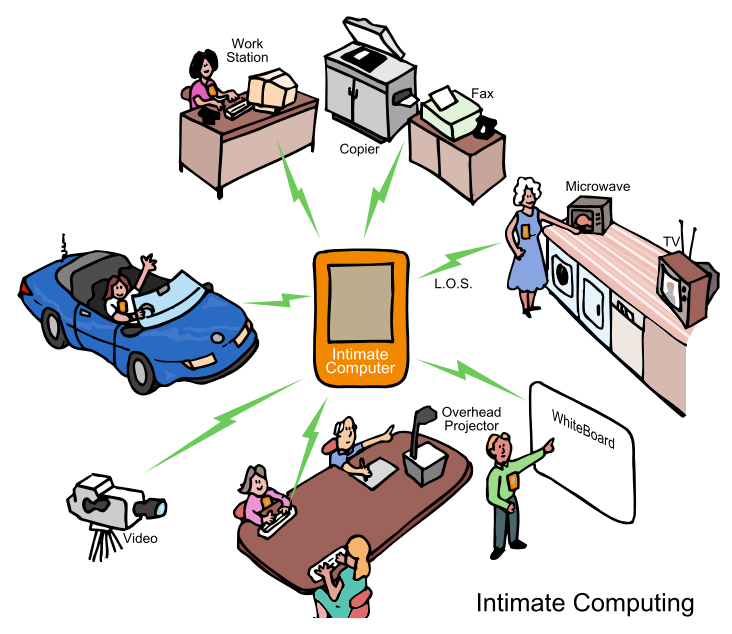
\includegraphics[scale=0.6]{pics/intimate_computing}
\caption{Intimate Computing Simple Model \cite{lamming1994forget}}\label{fig:intimate_computing}
\end{centering}
\end{figure}

\textit{\textbf{Summary}}: To sum up, in this section we have decided to include historical contexts as tags associated with the contacts because they are highly valuable information and according to Whittaker et. al: whether a contact is important to a user or not largely depends on the \textit{history of their prior interactions} \cite{Whittaker2002}. After investigating the design principles of context-aware systems and Forget-me-not, it is our conclusion that some important aspects should be apply to our context-aware Contact application as follows:

\begin{itemize}
    \item \textit{Internal vs. External Context}: External contexts being easier to capture, our plan is to focus on external contexts like date/time and location first. After that, we will try to extract internal context by accessing users' call logs, instant messages, emails and so on.
    \item \textit{Data Capturing Methods}: The core of our system lays on the mobile phones with many available sensors like GPS, accelerometer, gyroscope. The operating systems of modern mobile phones allow applications to access the data gathered by those sensors directly so the capturing method we will mainly use is \textit{Direct sensor access}.
    \item \textit{Logical Architecture}: Following the architecture described by Ailisto et. al., our system will use four layers: Sensors, Raw data retrieval, Storage/management, and Application. The Preprocessing layer is omitted like the majority of context-aware systems. Regarding the Sensors layer, we will take a step-by-step approach by utilizing the physical sensors at the beginning then moving on to explore applicable virtual sensors later. Notably, many elements of these layers have already been implemented by the mobile phone's operating system. We can take advantage of that and focus on building the application.
    \item \textit{Context Model}: We choose the key-value model because of its simplicity and high efficiency. The contexts we capture will be stored as numerous tags. The tags should be small and easy to search, retrieve, create, etc. Therefore, the key-value model is definitely one of the best choices for us.
    \item \textit{Lessons from Forget-me-not Project}: What we are trying to do can be considered a small version of Intimate Computing. Our novel Contacts application will be a memory aid device which can help users find the name of a forgotten contact through the events having happened around him/her in the past or through the interaction history between the users and him/her. In the first phase, we will try to make our application collect some easy clues, activities which can help recall a contact like the date/time when the contact is created, the location when it happens. In future expansion, we will include more sophisticated clues like the event happening during the creation date, or the interactions between the users and the contacts.
\end{itemize}

\section{Contact Relationships}\label{contactrelationships}
There are various studies of the Contacts application from different aspects like improving the contact information, demoting unused/unimportant contacts. However, the relationships between contacts seem to have been forgotten by researchers. In our opinion, contact relationship is an important characteristic which need to be investigated. In this thesis, we introduce a novel internal network of contacts where each relationship between two contacts is an edge of the network graph. All contacts in a mobile Contacts application and the relationships between them form a big network which we call a ``Reversed Social Network''. There are two reasons why we call it a reversed social network. First, it shares the same features with a normal social network. Second, the content in it comes from a reversed point of view. In other words, while in a normal social network like Facebook the social profiles are created by the actual attendees, in a reversed social network the profiles are created by the network owner - the user of the Contacts/Phonebook application. In this section, we will investigate the definition of a social network site then compare the similarities/differences between a reversed social network and a normal one.

\subsection{Social Network Sites: Definition and History}
Social network sites have been growing enormously, attracting hundreds of millions of users all over the world. In their work ``Social Network Sites: Definition, History, and Scholarship'' \cite{boyd2010social} Boyd and Ellison defined social network sites as web-based services which allow people to:

\begin{enumerate}
  \item Build a public or semi-public profile in their bounded system.
  \item Establish a list of other users who they have a connection with.
  \item Explore and traverse their connection list and other users' list within the system.
\end{enumerate}

Social network sites are unique not because they help people to meet new friends, but rather that they allow users to establish their own existing social networks online. Sometimes new connections between strangers are created but that is normally not the main goal. Connections in a social network site are often formed between participants who share some offline connections.

Although different social network sites have different features, the majority of them possesses a backbone of user profiles which illustrates a collected list of friends who are also users of that network. A profiles is a special page for an individual to ``type oneself into being'' \cite{sunden2003material}. Usually after joining a social network, a user is requested to fill out a form of questions. Then the answers in the form will be used to generate that person's profile page. Some typical questions ask about name, age, location, interests and a short description of the participant. People also have the option to upload a profile picture, and enhance their profiles by adding multimedia content. Profile visibility differs from site to site and according to user settings. By default, Facebook users can view other's profiles if they are directly connected, unless a user chooses to restrict his/her profile accessibility permission. On the contrary, LinkedIn decides what a user can access based on whether or not he/she has a paid account.

Many social network sites support a method for participants to leave messages on their friend's profile pages. This function often leads to another feature called leaving comments on these messages. Additionally, social networks usually have a private messaging system similar to email.

Besides user profiles, connections, comments, and private messages, social network sites differ vastly in functionalities and participants. Some sites have photos and videos sharing features while other ones have built-in blogging capability. A few social network sites are specified for mobile phones such as Dodgeball \cite{humphreys2007mobile}. However, most web-based social networks also support mobile devices with some limitation like Facebook, LinkedIn, MySpace. Several social network sites are designed for users in particular geographic regions and languages. There are also some social networks which target particular religious, ethnic, political, or other personality-driven groups. Furthermore, social networks for dogs and cats even exist and their owners will be the one who manage their pet's profile.

\begin{figure}[p]
\begin{centering}
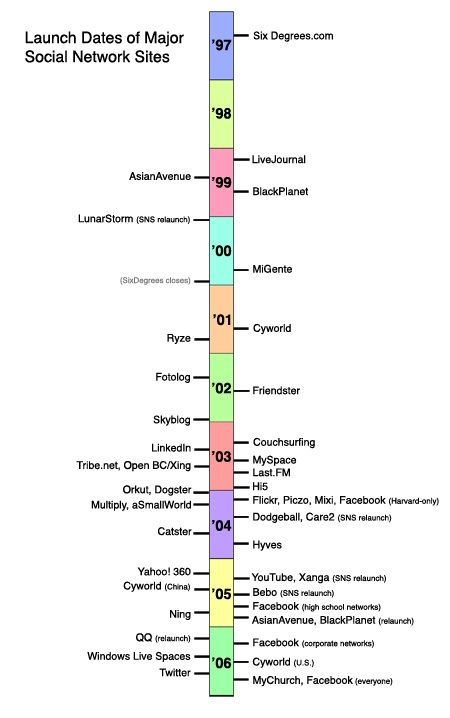
\includegraphics[scale=0.8]{pics/social_network_history}
\caption{Timeline of the launch dates of various major social network sites and dates when community sites re-launched with social network features \cite{boyd2010social}}\label{fig:social_network_history}
\end{centering}
\end{figure}

\subsection{Graphy vs. Social Network Sites}
\subsubsection{Similarities}
According to the definition from Boyd and Ellision above, Graphy can be considered a special type of social network:

\begin{enumerate}
    \item \textit{Building a public or semi-public profile in their bounded system}: Every record in a Contacts application is a profile of an individual. A contact profile and a social network profile are strikingly similar. They both consists of basic information about the person and a profile picture. The difference here is that the contact profiles are mostly private and only visible to the owner of the application.
    \item \textit{Establishing a list of other users who they have a connection with}: In Graphy, we connect the contacts with each other based on their real life relationship.
    \item \textit{Exploring and traversing their connection list and other users' list within the system}: The owner/user of Graphy can view and traverse the entire network of connections.
\end{enumerate}

From this comparison, we strongly believe that Graphy can stand out as another type of social network which may even evolve further like some other specialized services such as QQ, Cyworld, etc. QQ began as a Chinese instant messaging service which then developed into a major social network in China. Cyworld started as a Korean discussion forum, LunarStorm as a community website, Skyrock as a French blogging tool before including social network functionalities. Classmate.com was a school directory and started supporting friend list after social networks became widespread. All these services were founded and were based on functionalities not directly related to social network just like Graphy (based on Phonebook/Contacts application), then adapted to turn into full-feature social network sites.

\subsubsection{Differences}

\paragraph{Reversed Social Network}
The biggest difference between Graphy and a normal social network site like Facebook is the nature of the nodes and their connections in the networks. In a normal social network, a node is typically an user profile page which contains the information provided by that user. The connections between the nodes are established based on real life relationships which are also specified by the users. Therefore, the content of normal social networks comes from the ``first-person perspective'' or the owner of the nodes. On the contrary, in our Graphy system, the nodes are the contacts of the phone book/Contacts application. The information of the contacts as well as the relationships between them are determined by the owner of the phone book. In other words, the content of Graphy comes from the ``third-person perspective'' or the owner of the whole network.

\paragraph{Information Accuracy}
In online systems which allow people to freely assemble an online portrayal of self, there are several processes of impression management and self-presentation. Although most systems promote their users to create authentic representations of themselves, they usually do this to different degrees. In Friendster, an extremely popular social network site during the period between 2002 and 2007, many participants put incorrect information about themselves into their profiles. There were even profiles called ``Fakester'' which Boyd asserted that they never were real in her study \cite{boyd2010social}. Friendster was designed to only allow participants to view profiles of other users who were less than five degrees away. As a result, to extend their scope, people started adding acquaintances and strangers as friends so they can view more profiles. Some participants even tremendously collected friends. Not only serving the purpose of profiles viewing, the friends list was also an identity indicator of the profile owner. Consequently, people on social network sites had a high tendency to add interesting strangers into their circle of friends. Exploiting this trend, MySpace spammers created attractive fake profiles to collect targets for spamming. The problem of inaccurate friendships were emphasized even more in another study by Boyd \cite{boyd2006friends} in which she pointed out that friends on social network sites are not the same as friends in real life and online social network friends present to offer people imaginary audiences to guide behavioral norms. To sum up, in a normal social network, user profiles and the relationships between them do not have a high accuracy.

In Graphy, the contact profiles and their relationships are established by the information given by Graphy's users. Therefore, the data is much more reliable than the ones in normal social network. The only one case where Graphy's data is not accurate is when the users enter wrong information which is less likely to happen. Comparing with normal social network sites, Graphy content is not abundant, however, it is much more accurate, useful to the users, and more compact with less irrelevant data.

\paragraph{Relationship}
After joining a social network, people are regularly asked to find other users who they have a relationship with. However, these relationships often do not provide much information about the real-life relationship between them. The labels for these relationships vary from site to site, the common terms are ``Friends'', ``Contacts'', and ``Followers''. Almost all social network sites use bi-directional relationships. There are a few sites allowing one-directional connections which are often labeled as ``Followers'' or ``Fans'', but some of them just use the term ``Friends'' like the majority. Notably, the term ``Friends'' is sometimes misleading since the relationships do not necessarily imply normal real-life friendship and there are many reasons behind people's social network connections. For example, LinkedIn only uses plain connections, Facebook uses mostly ``Friends'' connections and a few special connections such as ``Father'', ``Mother'', ``Brother'', etc. Even though Facebook users can categorize their friends in different groups, it is still nearly impossible to describe a relationship like ``A is a student of B'', ``B is the professor of A'', etc. In a public environment like a social network, revealing these kinds of relationships may not be ideal since people more or less want to protect their privacy. In comparison, these types of relationships could be used frequently in a reversed social network where people can freely create these relationships between their contacts without any concerns of privacy.

%\paragraph{Friend Suggestion}
%
%In a social network, suggesting friends or groups to a user is essential. It helps users to expand their network to other people who share a mutual property such as interest, organization. While major social network like Facebook, LinkedIn, Google+ are doing well in suggesting people, none of the Contacts applications we have investigated has the suggesting ability. Ankolekar et. al.'s work \cite{Ankolekar2009} is the rare case that has made some effort in suggesting friends in a phone book environment. The authors built Friendlee, a mobile Contacts application which had the ability of browsing the friends of their close friends. Although Ankolekar et. al. applied a safeguard privacy for users to restrict visibility of chosen contacts to specific category of people, Friendlee still was not successful largely due to privacy reasons. Lederer et. al. study \cite{Lederer:2003:WKP:765891.765952} indicated that people may not be keen on sharing mobile contacts with others since the information is considered too personal. Consequently, suggesting friends in a Contact application environment is not favorable. However, internally suggesting relationships between contacts in a Contact application can be an applicable approach. When a user adds a contact to his/her phone book, the application can look into his existing contacts and past communication logs to find people who most likely have some relationship with this new one. In this way, all the information used to suggest connections comes from one user's Contact application, hence, there is no privacy issue.
% check this citation content Lederer

\paragraph{Privacy}
The arrival of social network sites have caused an increasing concern for internet privacy. Since social network sites promote information sharing and collaboration many people are giving their personal information out on the internet. These social network sites usually keep track of all user interactions. This behavior leads to a number of issues such as ``cyberstaking'', social profiling, and government surveillance. In one of the first scholarly research of privacy and social network \cite{gross2005information}, the researchers studied 4000 Carnegie Mellon University Facebook profiles. They revealed potential privacy threats contained in the personal information published by the students on Facebook, for example attackers could build up users' social security numbers from public information on their profile page. On the contrary, there is no privacy concerns in a reversed social network. In contrast with the public nature of a social network, the nature of a reversed social network is private. The reversed social network is made to provide information to the network's owner so there is little sharing in it. In the future version of Graphy, we plan to implement a contact sharing feature which allow a Graphy user to share his/her own contacts with another user. This type of sharing is controlled and limited hence we believe no privacy threat will be exposed. 

\paragraph{Bridging Online and Offline Social Networks}
An important aspect of social networks is that they support pre-existing social relations. Ellison et. al. \cite{ellison2007benefits} argue that Facebook helps its users maintain current offline relationships rather than meeting new friends. This is one of the main features which make social network sites stand out from earlier forms of public online community like forums and newsgroups. Many academic studies have been conducted on how online relations interact with offline ones. For example, Lampe et. al. \cite{lampe2006face} discovered that Facebook users spend much more time searching for someone they have an offline connection with than browsing for total strangers. Similarly, Boyd \cite{boyd2007youth} suggested that MySpace and Facebook allowed U.S. youngsters to socialize with their friends even when they are unable to meet each other. 

Being a reversed social network, Graphy also assists pre-existing offline connections. A relationship between two of Graphy's contacts represent their real-life connection. Moreover, a contact in Graphy should be someone the Graphy user needs to communicate with. Looking at this angle, Graphy connects the online and offline worlds even stronger than a normal social network does. The relationships in a normal social network are often weak ties \cite{boyd2010social} since a user's friend list often consists of many friends of friends, and people with some weak offline connections like being in the same organization. On the other hand, Graphy users generally just add a contact if they want to keep in touch with that person, this behavior indicates a stronger relationship.

\section{Cloud-based Contacts Application}\label{cloudcontact}
\subsection{Overview of Cloud Computing}
Cloud computing has been an evolving trend in the computing world recently. According to the U.S. National Institute of Standards and Technology \cite{mell2011nist}, cloud computing is a model which facilitates convenient, ubiquitous, and on-demand network access to computing resources. The model consists of five fundamental characteristics, three service models, and four deployment models.

\subsubsection{Fundamental Characteristics}

\begin{itemize}
    \item \textit{On-demand self-service}: Users can independently control computing power as they need without directly contacting the service providers.
    \item \textit{Broad network access}: The services are accessible over the network through miscellaneous platforms like personal computers, laptops, phones, and tablets.
    \item \textit{Resource pooling}: The service providers' resources are pooled. According to user usage, physical and virtual resources are dynamically allocated.
    \item \textit{Rapid elasticity}: The service providers can plan and supply computing capabilities in an elastic way to scale back and forth regarding consumer demands. From the user point of view, the capabilities seem to be unlimited and are ready at any time.
    \item \textit{Measured service}: The resources can be controlled, monitored, and optimized automatically by the cloud system.
\end{itemize}

\subsubsection{Service Models}

\begin{itemize}
    \item \textit{Software as a Service (SaaS)}: The users consume the service by using the providers' applications. The applications can be provided through different interfaces like personal computer programs, mobile apps, or web browsers. All the underlying infrastructures like hardware, network, operating system and configuration are totally hidden from the end users.
    \item \textit{Platform as a Service (PaaS)}: The users consume the service by implementing applications onto the cloud infrastructure using libraries and tools supplied by the service providers. Underlying infrastructures like hardware, network, and operating system are hidden from the users but they can control the configuration settings of the application environment.
    \item \textit{Infrastructure as a Service (IaaS)}: The users consume the service by using the fundamental computing resource like processing power, storage to deploy and run any software. Underlying infrastructures like hardware and network are hidden from the users but they can manage processing power, storage, operating systems and applications.
\end{itemize}

\subsubsection{Deployment Models}

\begin{itemize}
    \item \textit{Private Cloud}: The cloud infrastructure is provided to be used by a single organization. It could be owned and operated by that organization or a third party.
    \item \textit{Community Cloud}: The cloud infrastructure is provided to be used by a specific community which have some common interests. It could be owned and operated by the community or a third party.
    \item \textit{Public Cloud}: The cloud infrastructure is provided to be used by the public. It could be owned and operated by a company or an organization.
    \item \textit{Hybrid Cloud}: The cloud infrastructure is a combination of two or more of the above cloud models.
\end{itemize}

\subsection{Utilizing Cloud Computing in Contacts Applications}
Traditionally, database of a Contacts application lies in separated phones. It makes the process of transferring contacts from phones to phones really difficult and prone to inconsistent data. Nowadays, with the support of cloud computing, there are many cloud-based database services for contacts like Outlook Contacts, Gmail Contacts. These services give users a lot of benefits as below:

\begin{itemize}
   \item The ease to access contacts from anywhere
   \item Automatic synchronization contacts from phones to phones
   \item Backing up contacts
   \item Integrating phone book contacts with other services
\end{itemize}

Learning from that, we want our Graphy system to provide the same features. Unfortunately, all of the above services are closed source. Therefore, we have to develop our own communication and synchronization solution which will be discussed carefully in the Implementation section \ref{implementation}. Using cloud computing models and the trending RESTful communication technology, our solution makes it easy for users to work offline through a local database while maintaining a central cloud database to backup and synchronize data to other devices when needed. Our cloud service model and deployment model will be software-as-a-service and community cloud. At the experiment stage, our application is used only by some targeted users but in the future, it is our hope that we can expand it into a public cloud service.

%Nonetheless, if a user simultaneously uses more than one service, he/she has to deal with duplicate contact data. To tackle this problem, all popular Contacts applications provide a functionality which will suggest the users similar contact profiles from different services, thus, users can merge/link them to one contact. This functionality currently runs locally on the mobile phone while it could be performed on the cloud servers. There are many more potential tasks which can be done on cloud but still not yet been investigated.


%\section{Network Visualization}
%When you have a network of friends or contacts, the need of visualizing that network may rise. L. C. Freeman \cite{freeman2000visualizing} showed that visualizing is more than simply creating pictures. Images of social networks have provided investigator with new insights into network structure and have helped them communicate those insight with others. F. Viegas \cite{Viegas} suggested that visualization can be of interest not only to analysts and researchers but also to the people whose data is being analyzed. LinkedIn's project InMaps \cite{Inmaps} provides users a visual way to look at all their connections. As shown in Figure \ref{fg:inmaps}, InMaps creates a graph from a user's contacts, and the connections between these contacts. It tries to group people who share more connections into different clusters of the graph so the user can label these clusters with names. However, since LinkedIn uses only plain connections between contacts, the edges in this graph do not have any label.

%\begin{figure}[!h]
%\begin{centering}
%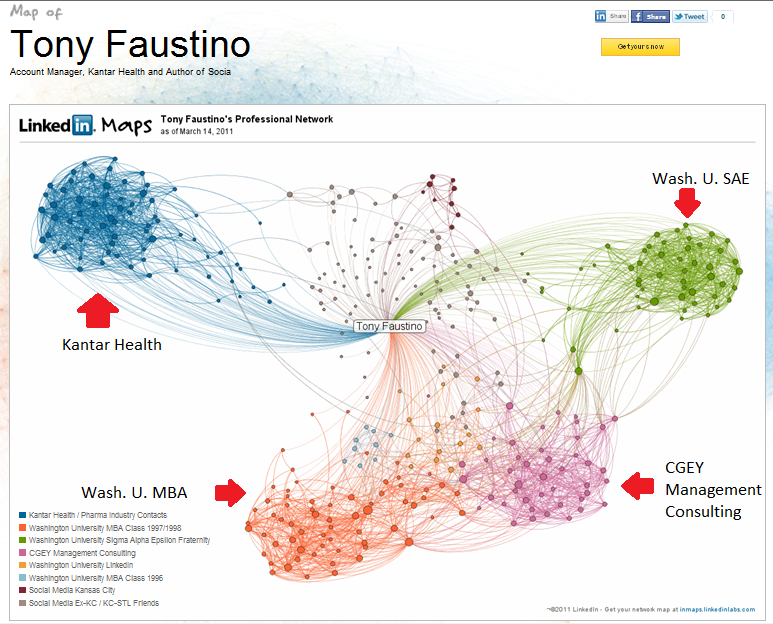
\includegraphics[scale=0.9]{pics/inmaps}
%\caption{LinkedIn Inmaps}\label{fg:inmaps}
%\end{centering}
%\end{figure}
